\section{Messergebnisse und Auswertung}

\subsection{Zählrohrcharakteristik mit \uran}
\label{sub:eval:uran}
Die gemessene Abhängigkeit der Zählrate $n$ von \uran ohne Untergrund von der Zählrohrspannung $U$ wird in der Abbildung \ref{img:char:uran} gezeigt.
\begin{figure}[H]
\begin{center}
  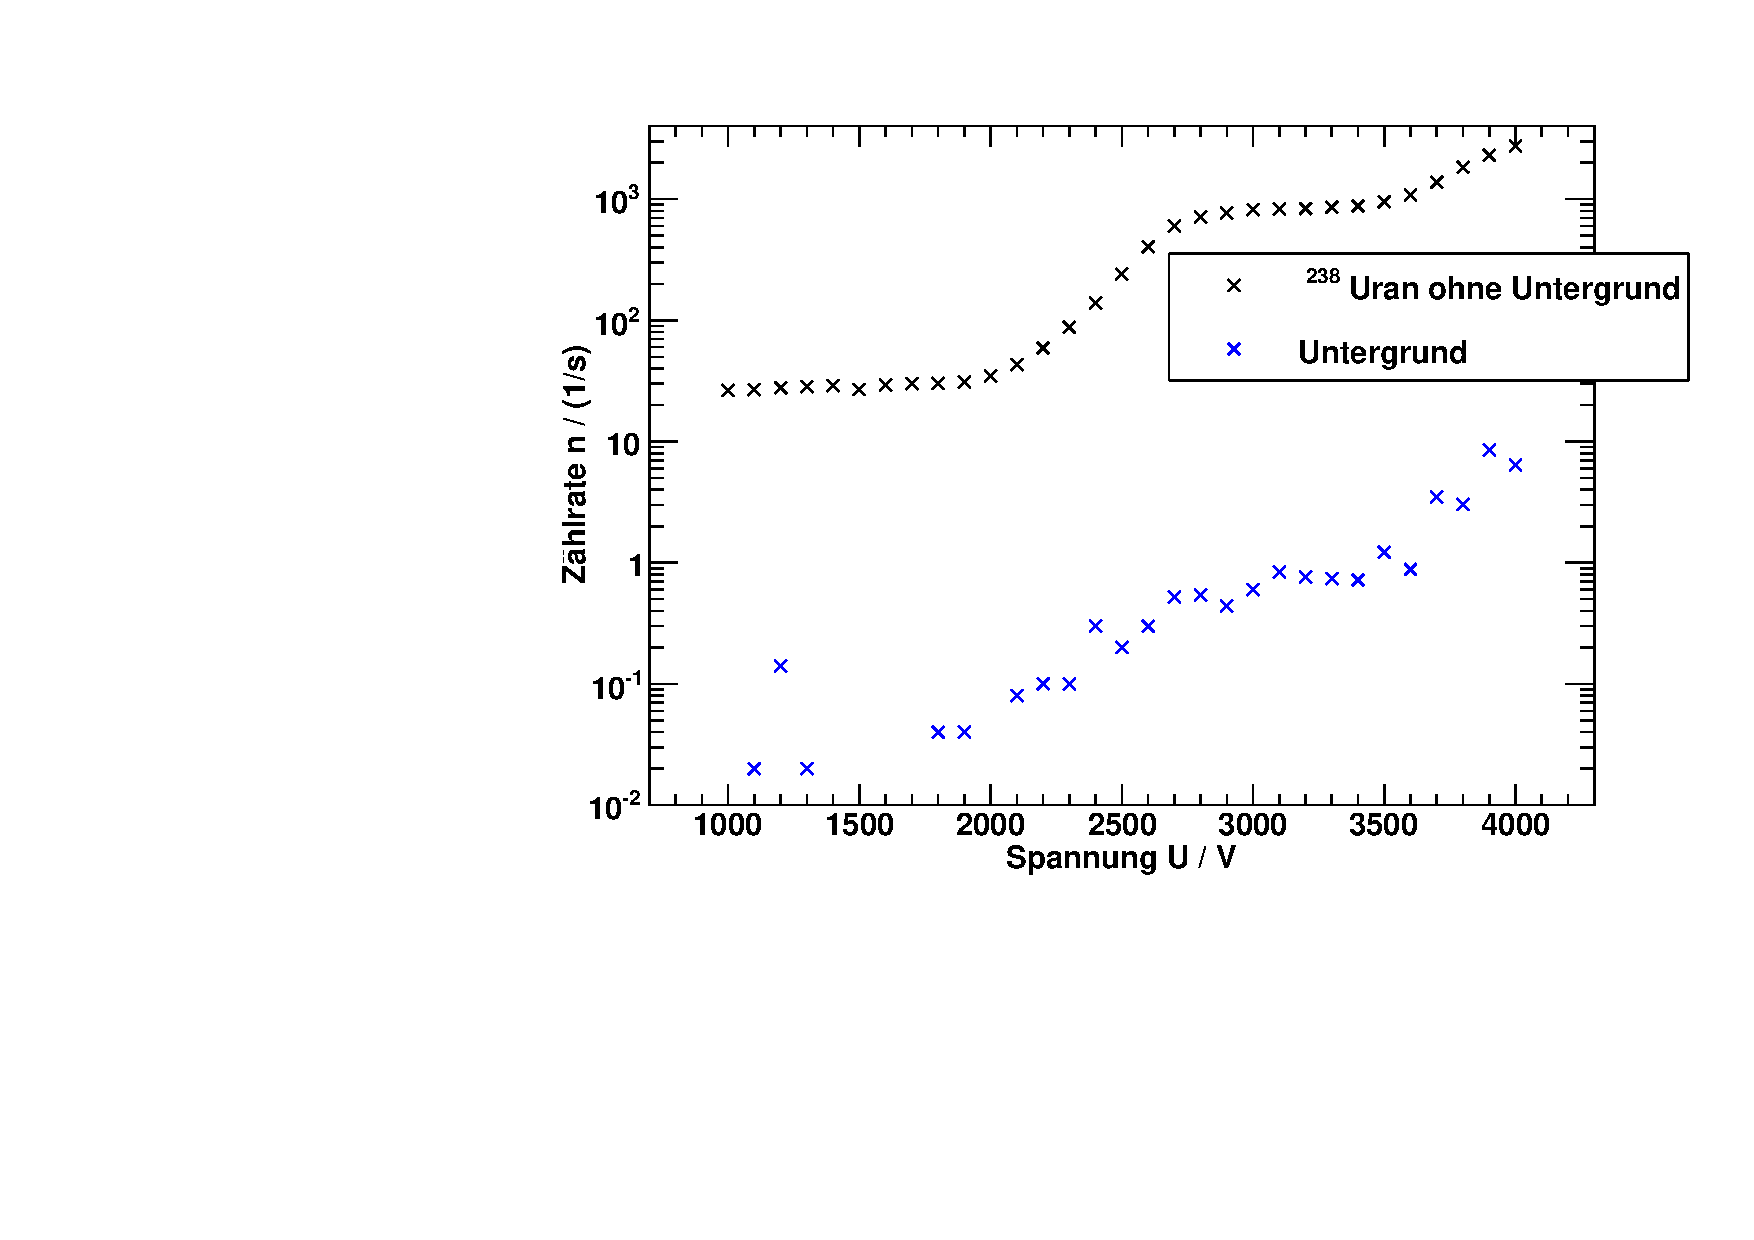
\includegraphics[width=15cm]{../img/Uran238_Charakteristik.pdf}
  \caption[Zählrohrcharakteristik mit \uran]{Zählrohrcharakteristik mit \uran und Untergrund}
  \label{img:char:uran}
\end{center}
\end{figure}
Man erkennt gut das $\alpha$-Plateau bis ca. $2000\,V$ und das $\beta$-Plateau von $2800\,V$ bis $3500\,V$, welche durch die 
unterschiedlichen Energien der beiden Strahlungen verursacht werden. Des weiteren wurde die Zählrate des Untergrundes in der gleiche Abbildung 
\ref{img:char:uran} abgebildet. Der Anstieg der Zählrate des Untergrundes, verursacht von der Zählrohrspannung, lässt sich gut erkennen. Allerdings 
sieht man auch die statistischen Schwankungen in der Zählrate des Untergrundes (die Messpunkte mit $n = 0 / s$ lassen sich auf der logarithmischen 
Skala nicht darstellen), da die einzelnen Messpunkte nur in einer geringen Zeitspanne ($t=50s$) aufgenommen wurden. Für eine glattere Kurve wäre 
eine längere Messzeit erforderlich gewesen. \\
Die relativen Fehler auf die gemessenen Zählraten $\hat{n}$ beträgt nach \autoref{eq:counts:errors}
\begin{equation}
  \frac{s_{\hat{n}}}{\hat{n}} = \frac{1}{\sqrt{\hat{n} \cdot t_{\hat{n}}}}
\end{equation}
Von der gemessenen Zählrate $\hat{n}$ zieht man die Untergrundszählrate $u$ ab, um die echte Zählrate $n$ zu berechnen.
\begin{equation}
  n = \hat{n} - u
\end{equation}
Der absolute Fehler von der echten Zählrate lässt sich folgendermaßen bestimmen.
\begin{equation}
  s_n = \sqrt{s_{\hat{n}} + s_u}
\end{equation}
Jedoch kann man die Fehler der Zählrate des Urans wegen der logarithmischen Skala nicht mehr gut erkennen, weshalb sie in der Abbildung 
weggelassen wurden.

\subsection{Bestimmung der Halbwertszeit von \samarium}
\begin{figure}[H]
\begin{center}
  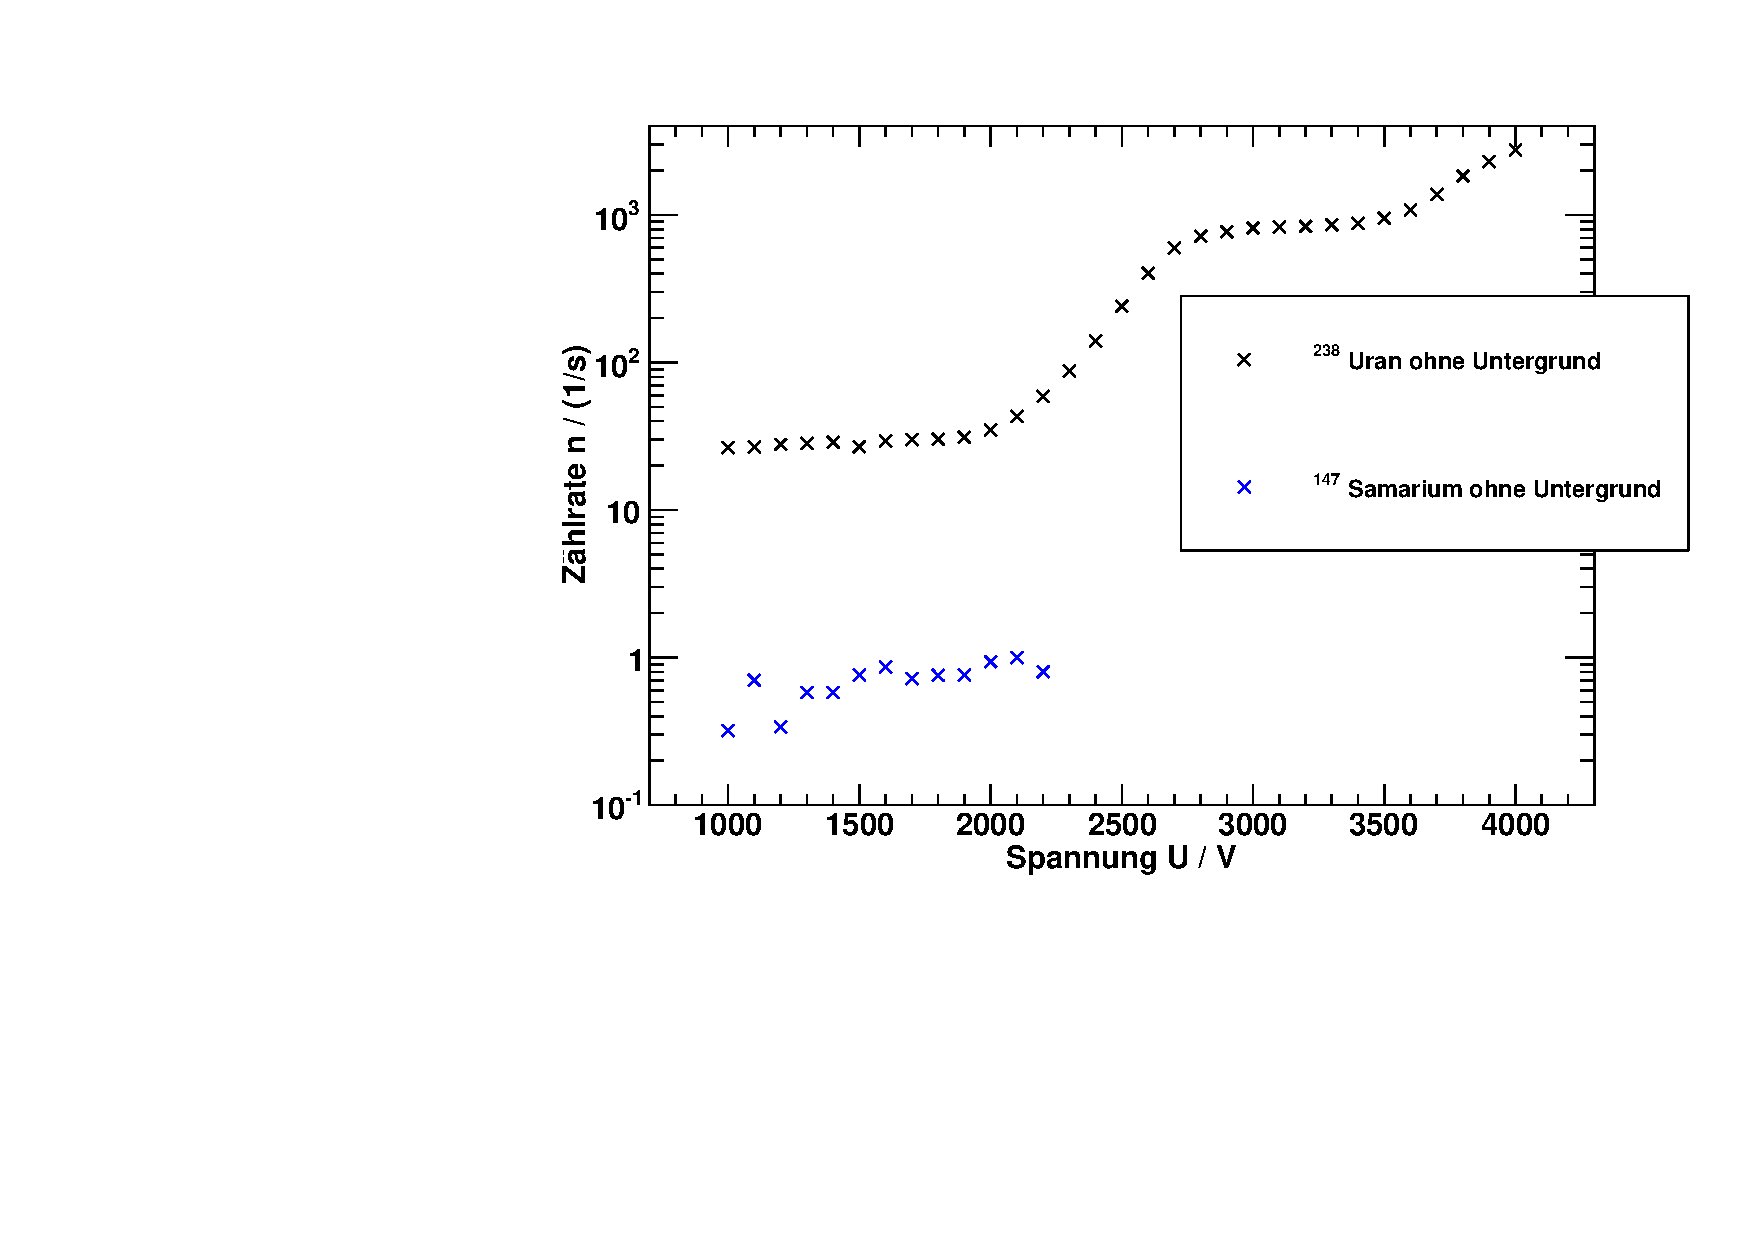
\includegraphics[width=15cm]{../img/Samarium147_Charakteristik.pdf}
  \caption[$\alpha$-Plateau mit \samarium]{$\alpha$-Plateau von \samarium} %TODO bessere beschreibung
  \label{img:char:samarium}
\end{center}
\end{figure}

\begin{figure}[H]
\begin{center}
  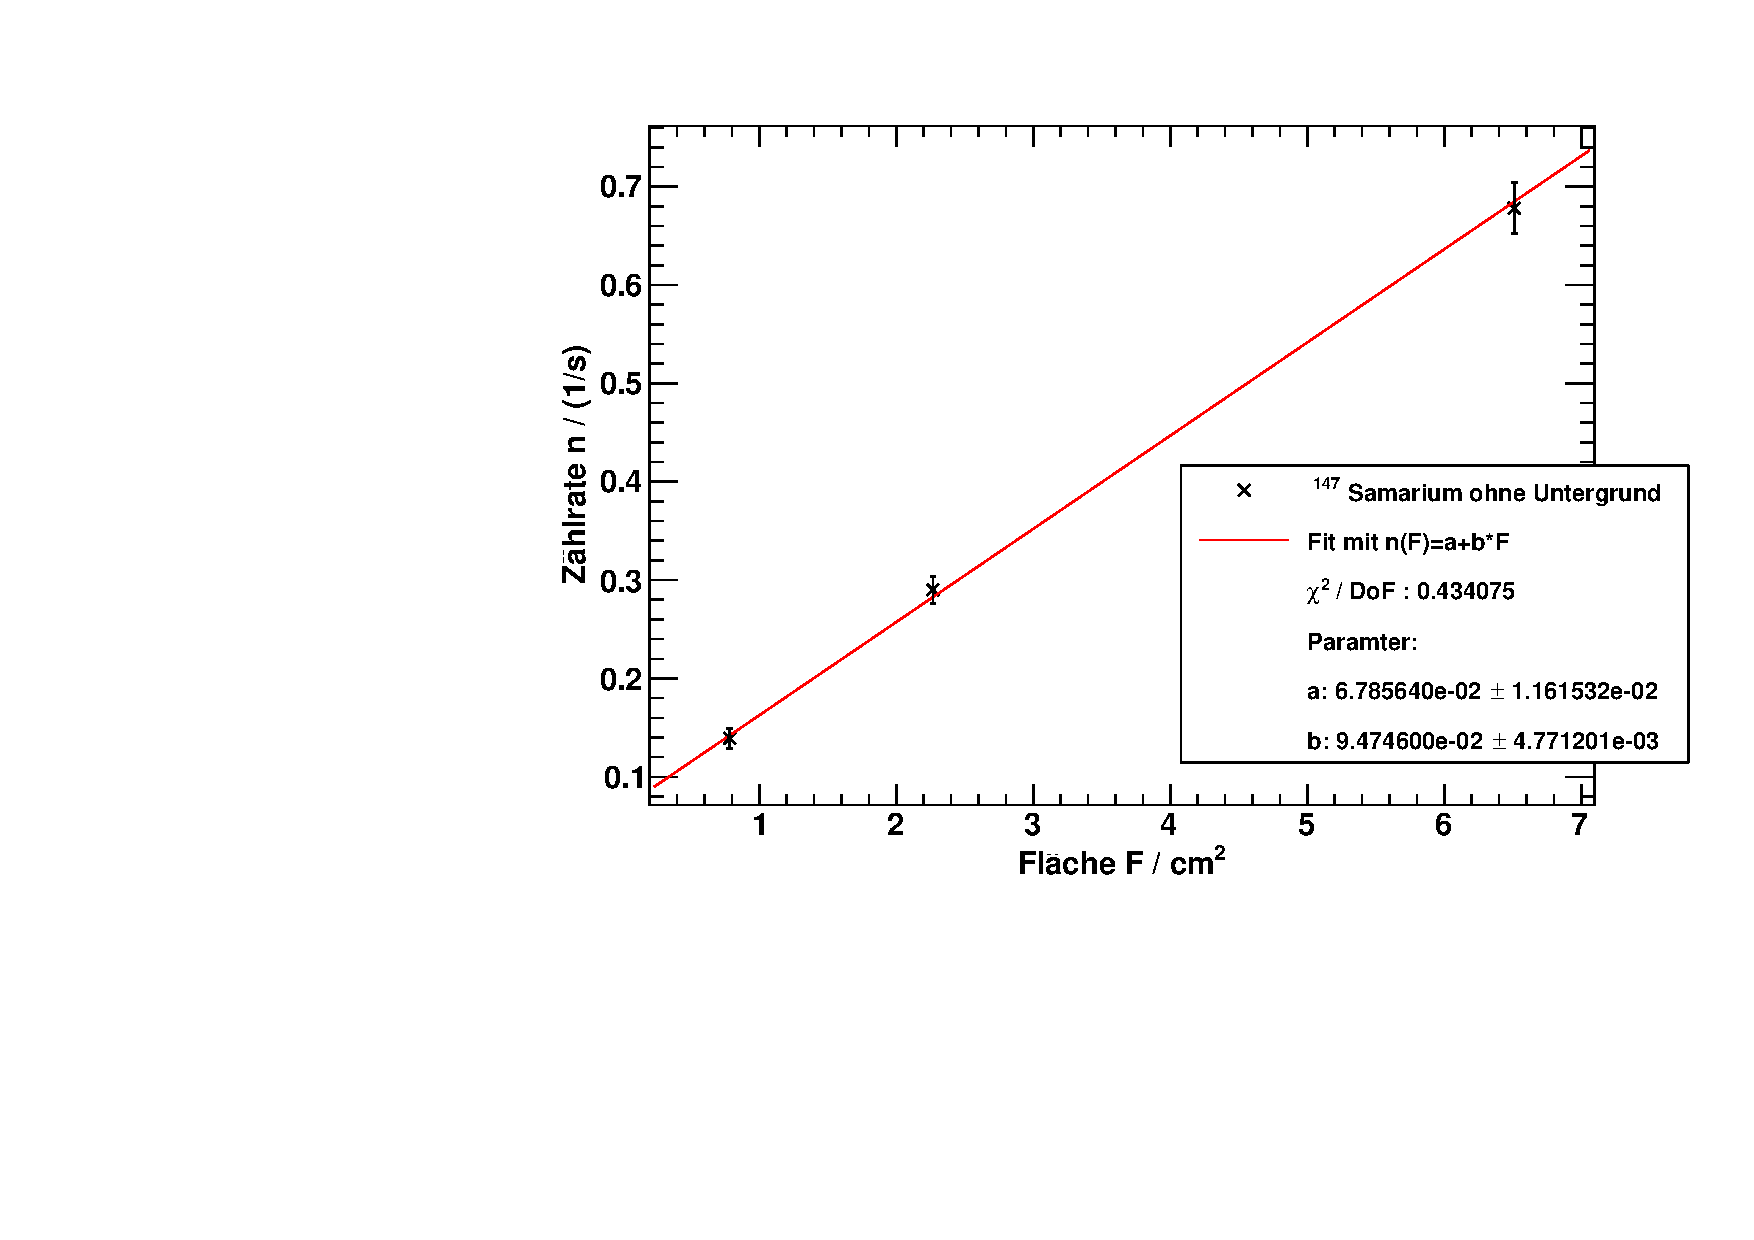
\includegraphics[width=15cm]{../img/Samarium147-Flaechenabhaengigkeit.pdf}
  \caption[Flächenabhängigkeit von \samarium]{Flächenabhängigkeit von \samarium bei 1600V}
  \label{figureLabel}
\end{center}
\end{figure}


%TODO Rest der Samariumauswertung

\subsection{Bestimmung der Halbwertszeit von \kalium}
\subsubsection{$\beta$-Plateau von \kalium}
\begin{figure}[H]
\begin{center}
  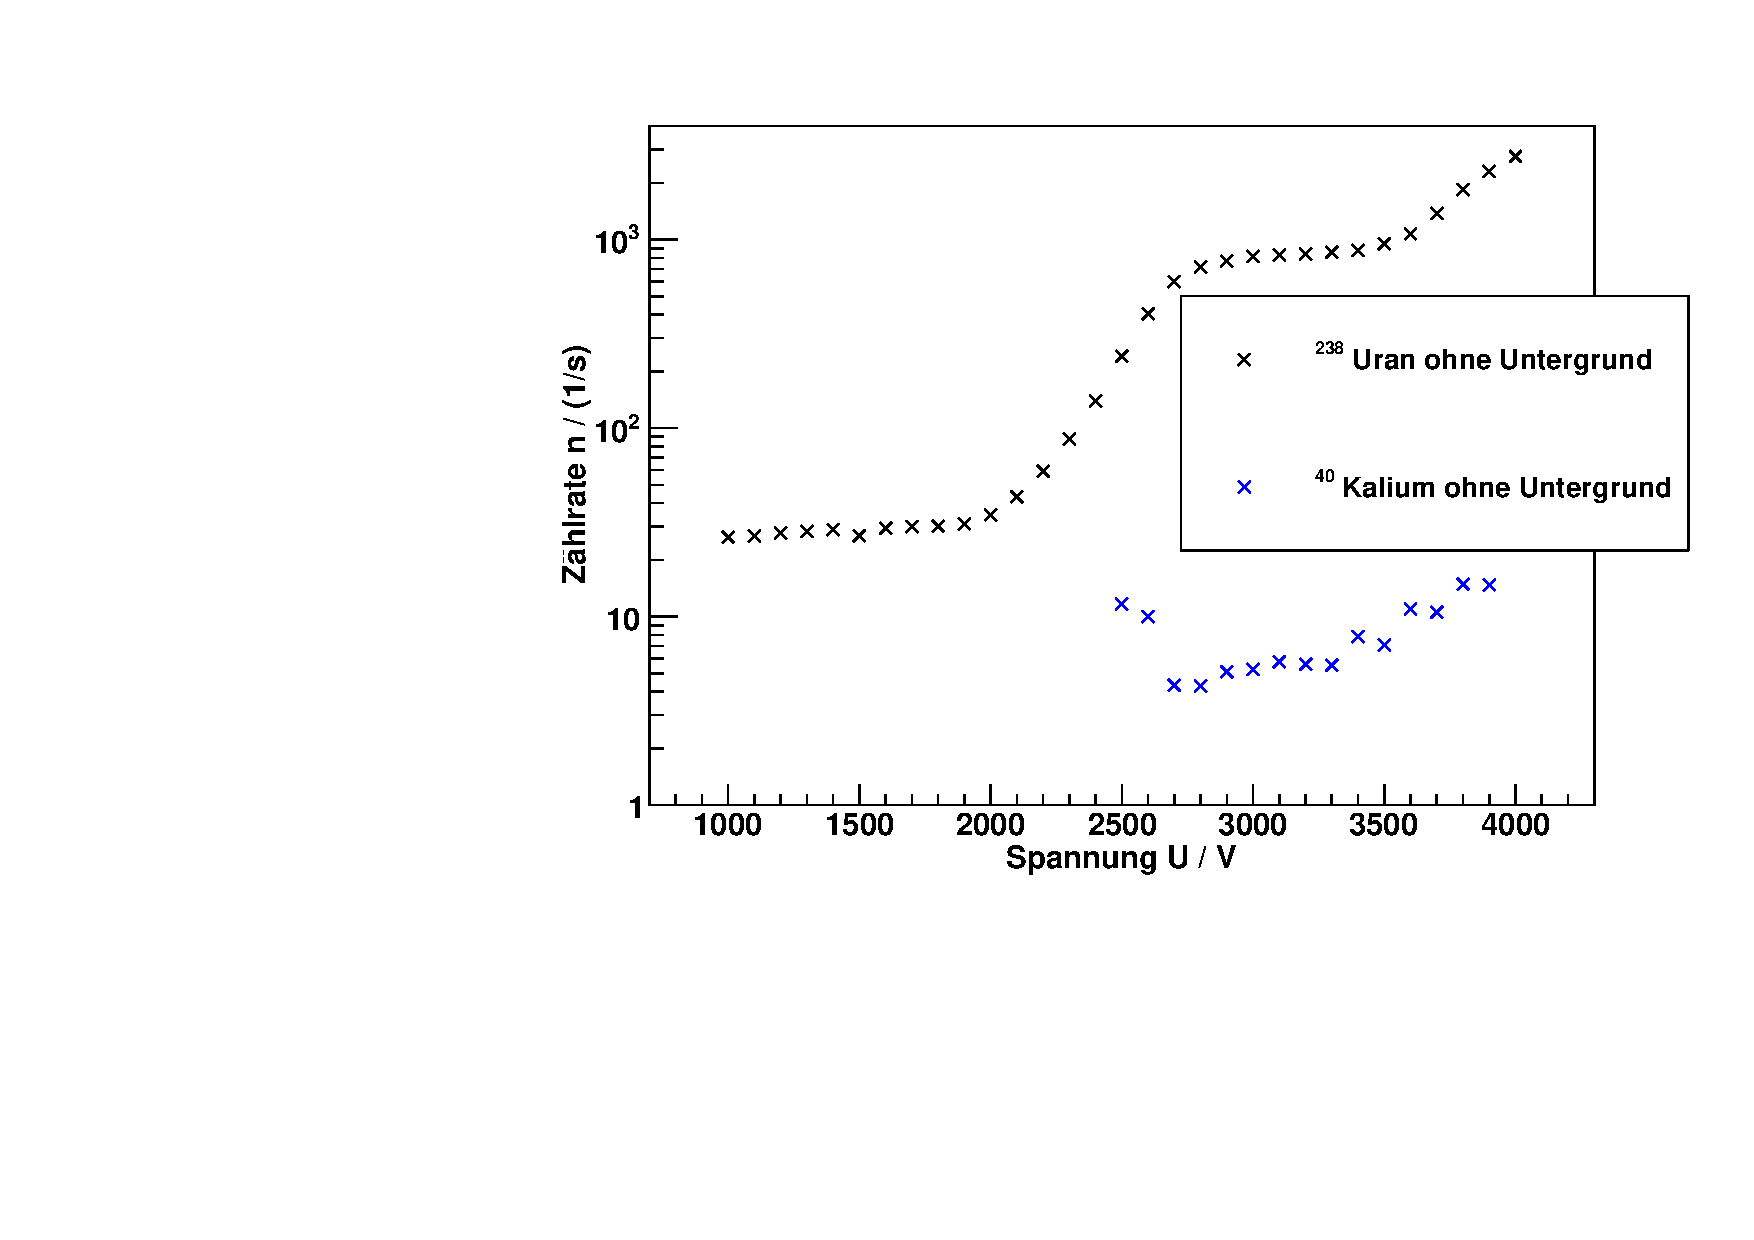
\includegraphics[width=15cm]{../img/Kalium40_Charakteristik.pdf}
  \caption[$\beta$-Plateau mit \samarium]{$\beta$-Plateau von \kalium}
  \label{img:char:kalium}
\end{center}
\end{figure}
In \autoref{img:char:kalium} ist das $\beta$-Plateau der Zählrate $n$ von \kalium ohne Untergrund gegen die Zählrohrspannun $V$ aufgetragen 
und in Vergleich mit der Zählrate von \uran gesetzt worden. Die Fehler wurden, wie in Kapitel \ref{sub:eval:uran} beschrieben, bestimmt.
%TODO Erklärung Peak am Anfang

\subsubsection{Massenabhängigkeit der Zählrate} %TODO besserer Titel?
Nach \autoref{eq:kalium:countrate} hängt die Zählrate folgendermaßen von der Masse der Probe ab:
\begin{equation}
  n(m) = \frac{f}{2} \frac{A_s \cdot F \cdot \rho}{\mu} \left( 1 - e^{- \frac{\mu \cdot m}{F \cdot \rho}} \right) = a(1-e^{-b \cdot m})
\end{equation}
mit
\begin{equation}
  a = \frac{f}{2} \frac{A_s \cdot F \cdot \rho}{\mu} \qquad \text{und} \qquad b = \frac{\mu}{F \cdot \rho}
\end{equation}
Die beiden Parameter $a$ und $b$ lassen sich mit einer Kurvenanpassung (siehe \autoref{img:kalium:massdep}) bestimmen. \\
Die Werte dafür sind in \autoref{tab:data:kalium} aufgelistet.
\begin{table}[H]
\caption{Z"ahlraten von \kalium\,f"ur verschiedene Massen mit Fehlern}
\begin{center}
\begin{tabular}{|c|c|c|c|}
  \hline
  Masse $m /$g & $s_m /$g & Z"ahlrate $n / (1/\text{s})$ & $s_n / (1/\text{s})$ \\ \hline 
  2.012 & 0.001 & 5.426 & 0.173 \\ \hline
  2.012 & 0.001 & 5.088 & 0.171 \\ \hline
  1.905 & 0.001 & 5.192 & 0.171 \\ \hline
  1.681 & 0.001 & 5.297 & 0.172 \\ \hline
  1.483 & 0.001 & 4.773 & 0.168 \\ \hline
  1.295 & 0.001 & 4.961 & 0.165 \\ \hline
  1.099 & 0.001 & 4.525 & 0.162 \\ \hline
  0.809 & 0.001 & 4.344 & 0.157 \\ \hline
  0.695 & 0.001 & 3.803 & 0.154 \\ \hline
  0.501 & 0.001 & 3.251 & 0.146 \\ \hline
  0.303 & 0.001 & 2.280 & 0.138 \\ \hline
\end{tabular}
\end{center}
\label{tab:data:kalium}
\end{table}
 
\begin{figure}[H]
\begin{center}
  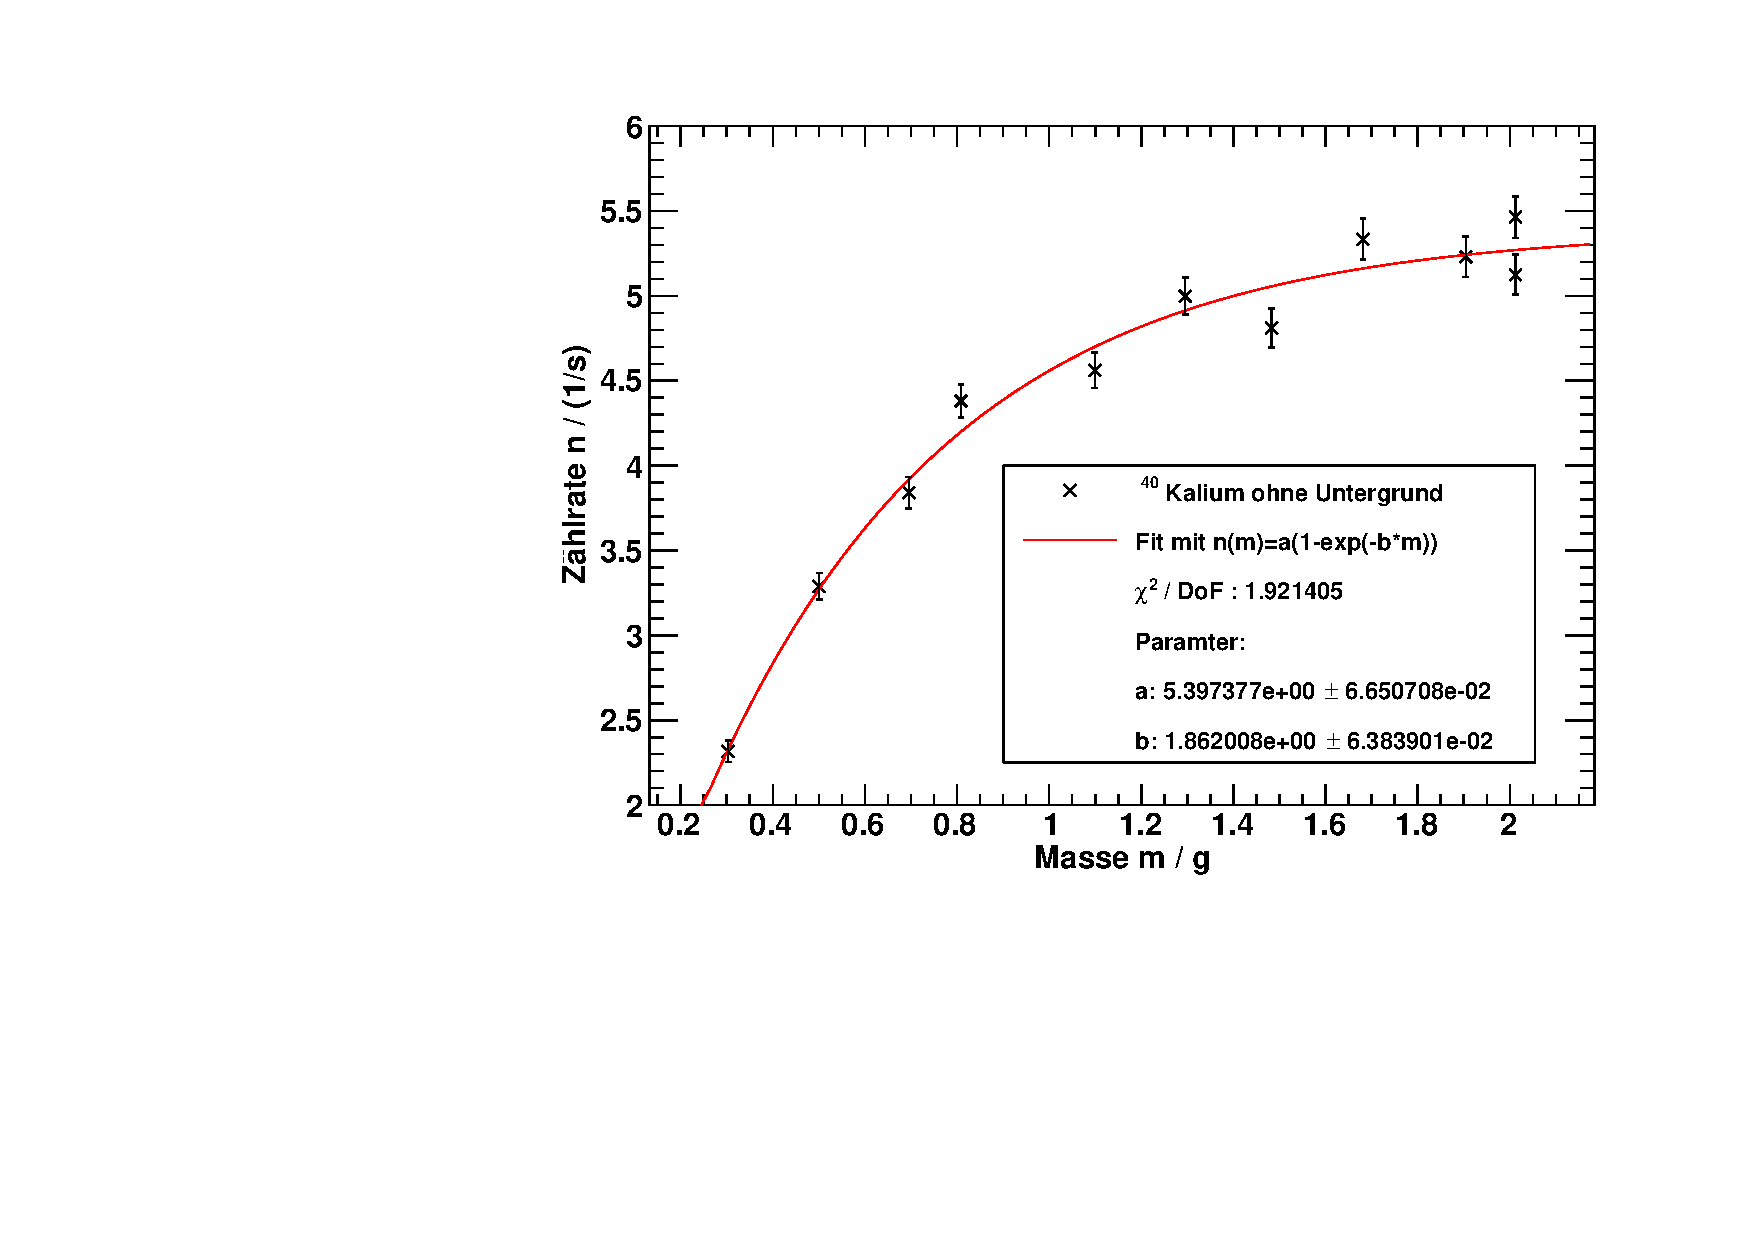
\includegraphics[width=15cm]{../img/Kalium40_Massenabhaengigkeit.pdf}
  \caption[Massenabhängigkeit der Zählrate von \kalium]{Massenabhängigkeit der Zählrate von \kalium bei 3200V}
  \label{img:kalium:massdep}
\end{center}
\end{figure}
Die Werte lauten:
\begin{gather}
  a = (5.397 \pm 0.067) \cdot \frac{1}{s} \\ %TODO runden ja oder nein?
  b = (1.862 \pm 0.064) \cdot \frac{1}{g} 
\end{gather}
Außerdem ergibt sich ein Korrelationskoeffizient von
\begin{equation}
  \rho = \frac{\cov(a, b)}{\sigma_a \sigma_b} = -0.82
\end{equation}
%TODO Chi^2 / DoF Auswertung

\subsubsection{Berechnung der Halbwertszeit}
Aus dem Produkt der beiden Parameter lässt sich die spezifische Aktivität $A_s = \frac{A}{m}$ bestimmen:
\begin{equation}
  A_s = \frac{2 \cdot a \cdot b}{f} \quad \Rightarrow \quad A = m \cdot \frac{2 \cdot a \cdot b}{f}
\end{equation}
Die Halbwertszeit von Kalium lässt sich nach \eqref{eq:kalium:halflife} mit %TODO refeq
\begin{equation}
  T_{1/2}({}^{40}K) = \frac{\ln 2}{1.12} \frac{N}{A}
\end{equation}
bestimmen. \\
Die Anzahl $N$ der Kaliumkerne in Kaliumchlorid ist:
\begin{equation}
  N = \frac{m \cdot N_A}{M_{KCl}} h_{\text{rel}}
\end{equation}
wobei $N_A$ die Avogadrokonstante, $M_{KCl}=74.5483\,u$ die molare Masse von Kaliumchlorid und $h_{\text{rel}}=0.0118\%$ die relative Anzahl von Kaliumkernen 
in Kaliumchlorid ist. \\
Daraus berechnet sich die Halbwertszeit von Kalium mit:
\begin{equation}
  T_{1/2} \left( {}^{40} K \right)  = \frac{\ln 2}{1.12} \frac{N_A \cdot h_{\text{rel}}}{M_{KCl}} \frac{f}{2} \frac{1}{a \cdot b} = const. \cdot \frac{1}{a \cdot b}
\end{equation}
Der Fehler ergibt sich aus den relativen Fehlern von $a$ und $b$ und der Berücksichtigung des Korrelationskoeffizienten $\rho$:
\begin{equation}
  \sigma_{T_{1/2}} = \sqrt{ \left( \frac{\sigma_a}{a} \right)^2 + \left( \frac{\sigma_b}{b} \right)^2 + 2 \cdot \frac{\sigma_a}{a} \cdot \frac{\sigma_b}{b} \cdot \rho   }
\end{equation}
Man erhält folgendes Ergebnis:
\begin{equation}
  T_{1/2} \left( {}^{40} K \right) = (1.20 \pm 0.03) \cdot 10^9\,a  
\end{equation}

\subsubsection{Diskussion des Ergebnisses}

%Tabellen mit Messergebnissen
%Abbildungen
%Auswertung, in der die Analyse der Messdaten beschrieben wird und die Ergebnisse mit ihren Fehlern zusammengestellt werden.